\documentclass[a4paper,12pt]{article}
\usepackage{codeanatomy}
\usepackage{pgfplotstable}
\pgfplotsset{compat=1.18}
\usepackage{multicol}
\usepackage{booktabs}
\usepackage{amsmath}
\usepackage{graphicx}
\usepackage{float}
\usepackage{listings}
\usepackage{mathtools}
\usepackage[thinc]{esdiff}
\usepackage[T2A]{fontenc} 
\usepackage[utf8]{inputenc}
\usepackage{titlesec, titletoc} 
\usepackage{cmap} 
\usepackage[english,russian]{babel} 
\usepackage{caption}
\usepackage{xcolor} 
\usepackage{geometry}
    \geometry{left=30mm, right=20mm, top=20mm, bottom=20mm}

\titlespacing*{\section}{0pt}{2\baselineskip}{\baselineskip}
\titlespacing*{\subsection}{0pt}{2\baselineskip}{\baselineskip}
\titlespacing*{\subsubsection}{0pt}{2\baselineskip}{\baselineskip}


\definecolor{codegreen}{rgb}{0,0.6,0}
\definecolor{codegray}{rgb}{0.5,0.5,0.5}
\definecolor{codepurple}{rgb}{0.58,0,0.82}
\definecolor{backcolour}{rgb}{0.95,0.95,0.92}

\lstdefinestyle{mystyle}{
    backgroundcolor=\color{backcolour},   
    commentstyle=\color{codegreen},
    keywordstyle=\color{magenta},
    numberstyle=\tiny\color{codegray},
    stringstyle=\color{codepurple},
    basicstyle=\ttfamily\footnotesize,
    breakatwhitespace=false,         
    breaklines=true,                 
    captionpos=b,                    
    keepspaces=true,                 
    numbers=left,                    
    numbersep=5pt,                  
    showspaces=false,                
    showstringspaces=false,
    showtabs=false,                  
    tabsize=2
}

\lstset{style=mystyle}

\begin{document}

\noindent \textbf{ФИО:} Соловей Г.И. \hfill \textbf{Группа:} в5130904/30322

\section*{Работа №1. Ознакомление с основами векторной графики и получение
  навыков работы с базовыми функциями графического API и
  трехмерными графическими примитивами.}
\subsection* {Задание. Вариант 33}
Целью работы является ознакомление с основами векторной графики и получение
навыков работы с базовыми функциями графического API и трехмерными
графическими примитивами.
Требуется при помощи стандартных функций графической библиотеки
(OpenGL/WebGL/Vulkan) изобразить указанные объекты и произвести необходимые
преобразования.
\begin{enumerate}
    \item Изобразить каркасный чайник и поместить его в каркасный куб. Размеры и
          местоположение примитивов на экране задать самостоятельно.
    \item Повернуть чайник относительно начала координат на -30 градусов вокруг оси Х
    \item Изобразить конус и сферу, где вершина конуса является центром сферы.
    \item Переместить конус на dy=-30, масштабирование сферы с коэффициентом 1,5
\end{enumerate}
\newpage
\subsection* {Выполнение задания}
Для выполнения всех лабораторных работ по предмету было решено использовать стандартную библиотеку OpenGL v.4.2 для C++ для рендеринга,
библиотеку GLFW для создания и управления окном, а также ImGui для для легкой отрисовки простых элементов интерфейса.
Библиотеку GLUT (FreeGLUT) было решено не использовать, так как она предоставляет функции устаревшего на данный
момент пайплайна графической отрисовки (fixed-function pipeline). В современном OpenGL большая часть рендеринга
возлагается на видеокарту посредством шейдеров, чтобы минимизировать использование процессора в пайплайне отрисовки.

Разработанная библиотека представляет собой упрощённый графический движок,
реализующий базовые компоненты современного графического приложения: управление окном,
камерой и процессом рендеринга.
Для управления зависимостями используется пакетный менеджер Conan 2.0.

\subsubsection* {Класс приложения - Application}

Класс Application представляет собой центральный управляющий компонент графического приложения, реализующий шаблон Singleton (доступ через статический метод get() и запрещённое копирование/перемещение).

Он отвечает за:
\begin{enumerate}
    \item создание и настройку окна на базе GLFW (параметры задаются через with\_width, with\_height, with\_title);
    \item инициализацию графической подсистемы (init, init\_graphics);
    \item запуск основного цикла рендеринга (run\_graphics\_loop);
    \item управление текущей камерой сцены (current\_camera, set\_current\_camera);
    \item хранение и управление набором объектов сцены (m\_objects, методы add\_object и remove\_object).
\end{enumerate}
Дополнительно класс обрабатывает события изменения размера окна (framebuffer\_size\_callback) и выполняет освобождение ресурсов (cleanup, деструктор).

Таким образом, Application инкапсулирует жизненный цикл приложения, управление окном и координацию отрисовки всех объектов сцены.
\newpage
\subsubsection* {Класс камеры - Camera}

Класс Camera представляет собой компонент, отвечающий за формирование матриц вида и проекции, необходимых для отображения сцены.

Он поддерживает два типа проекции: перспективную и ортографическую (перечисление Projection), а создание объектов осуществляется через статические фабричные методы perspective и orthographic.

Основные функции класса:
\begin{enumerate}
    \item вычисление матрицы вида (view\_matrix) на основе позиции и точки наблюдения;
    \item вычисление матрицы проекции (projection\_matrix) в зависимости от выбранного типа проекции;
    \item хранение параметров камеры: положение, цель (target), угол обзора (fov), размеры области отображения, ближняя и дальняя плоскости отсечения.
\end{enumerate}
Класс предоставляет интерфейс для получения (get) и изменения (set) всех параметров камеры, что позволяет динамически настраивать параметры отображения сцены.

Таким образом, Camera инкапсулирует параметры наблюдателя и преобразования, необходимые для корректного отображения трёхмерной сцены на экран.

\subsubsection* {Классы объектов - Object, RenderObject, Mesh, OBJMesh}
Данные классы образуют иерархию объектов сцены и отвечают за обновление и отрисовку геометрии:

\begin{enumerate}
    \item Object — базовый абстрактный класс всех объектов сцены, задающий интерфейс обновления через метод tick, вызываемый каждый кадр.
    \item RenderObject — расширяет Object, добавляя поддержку трансформаций (позиция, масштаб, вращение) и низкоуровневых графических ресурсов (VAO/VBO/EBO), а также абстрактный метод render для отрисовки.
    \item Mesh — конкретизация RenderObject, реализующая отрисовку геометрии с использованием материала; хранит данные о вершинах/индексах и ссылки на uniform-переменные шейдера (матрицы модели, вида и проекции).
    \item OBJMesh — специализированный класс Mesh, загружающий геометрию из файлов формата OBJ, выполняющий обработку вершин (позиции, UV, нормали) и устранение дубликатов через хеш-таблицу.
\end{enumerate}

В совокупности, эта иерархия реализует полный цикл работы с объектами сцены: от абстрактного обновления логики до загрузки и отображения конкретной 3D-модели.


\subsubsection*{Класс материала объекта - Material}
Класс Material инкапсулирует работу с шейдерной программой и отвечает за создание, компиляцию и использование графических шейдеров.

Он обеспечивает:

\begin{enumerate}
    \item загрузку исходного кода вершинного и фрагментного шейдеров (в том числе из файлов через from\_files);
    \item компиляцию отдельных шейдеров и их линковку в единую программу (compile\_vertex, compile\_fragment, compile\_program);
    \item активацию шейдерной программы для использования при рендеринге (use);
    \item доступ к идентификатору GPU-программы (program).
\end{enumerate}

Дополнительно класс отслеживает корректность компиляции (is\_valid) и предоставляет подробную информацию об ошибках на каждом этапе (вершинный, фрагментный шейдер и итоговая программа).

Таким образом, Material абстрагирует низкоуровневую работу с OpenGL-шейдерами и обеспечивает удобное управление графическими эффектами при отрисовке объектов.

\newpage

\subsection* {Использование библиотеки для выполнения лабораторной работы}
В рамках данной работы библиотека используется как базовый каркас для создания и отображения трёхмерной сцены, позволяя сосредоточиться на генерации геометрии и взаимодействии с объектами.

Использование библиотеки включает следующие этапы:

\begin{enumerate}
    \item Инициализация приложения: через класс Application создаётся окно, настраиваются его параметры и запускается основной цикл рендеринга.
    \item Создание материалов: с помощью класса Material загружаются и компилируются шейдерные программы, которые определяют внешний вид объектов.
    \item Формирование сцены: используются как встроенные (OBJMesh для загрузки модели чайника), так и пользовательские классы (Cube, Sphere, Cone), унаследованные от Mesh, в которых реализуется генерация геометрии.
    \item Управление объектами: каждому объекту задаются трансформации (позиция, масштаб, поворот), после чего они автоматически включаются в цикл отрисовки.
    \item Настройка камеры: через Application осуществляется доступ к текущей камере, параметры которой (позиция, направление, угол обзора) изменяются в процессе выполнения.
    \item Интерактивное управление: с использованием ImGui реализован пользовательский интерфейс (UI), позволяющий в реальном времени изменять параметры камеры, переключать режим отображения (каркасный/сплошной) и модифицировать параметры сцены.
\end{enumerate}

Таким образом, библиотека обеспечивает полный цикл работы приложения — от инициализации графического контекста до интерактивного управления сценой, в то время как основное внимание в работе уделяется реализации и настройке трёхмерных примитивов.
\newpage
\subsection*{Скриншоты работы приложения}

\begin{figure}[H]
    \centering
    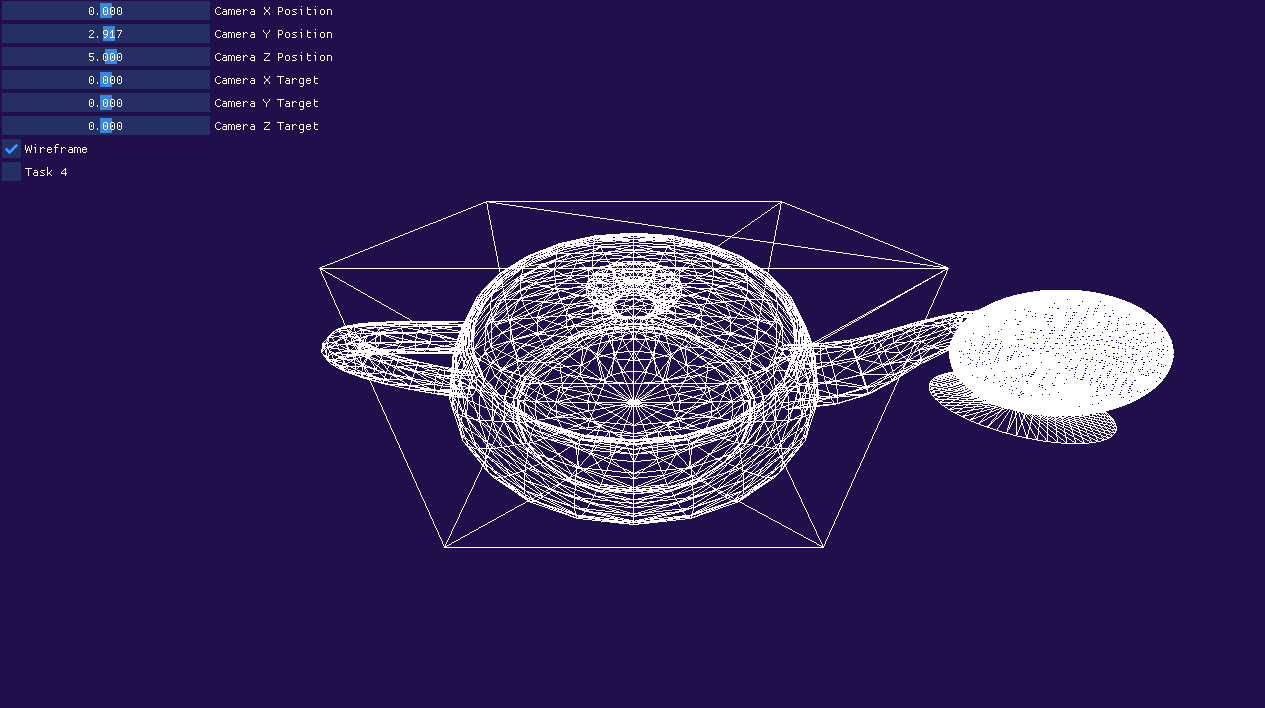
\includegraphics[width=\textwidth]{images/image.png}
    \caption{Первичная сцена приложения}
\end{figure}
\begin{figure}[H]
    \centering
    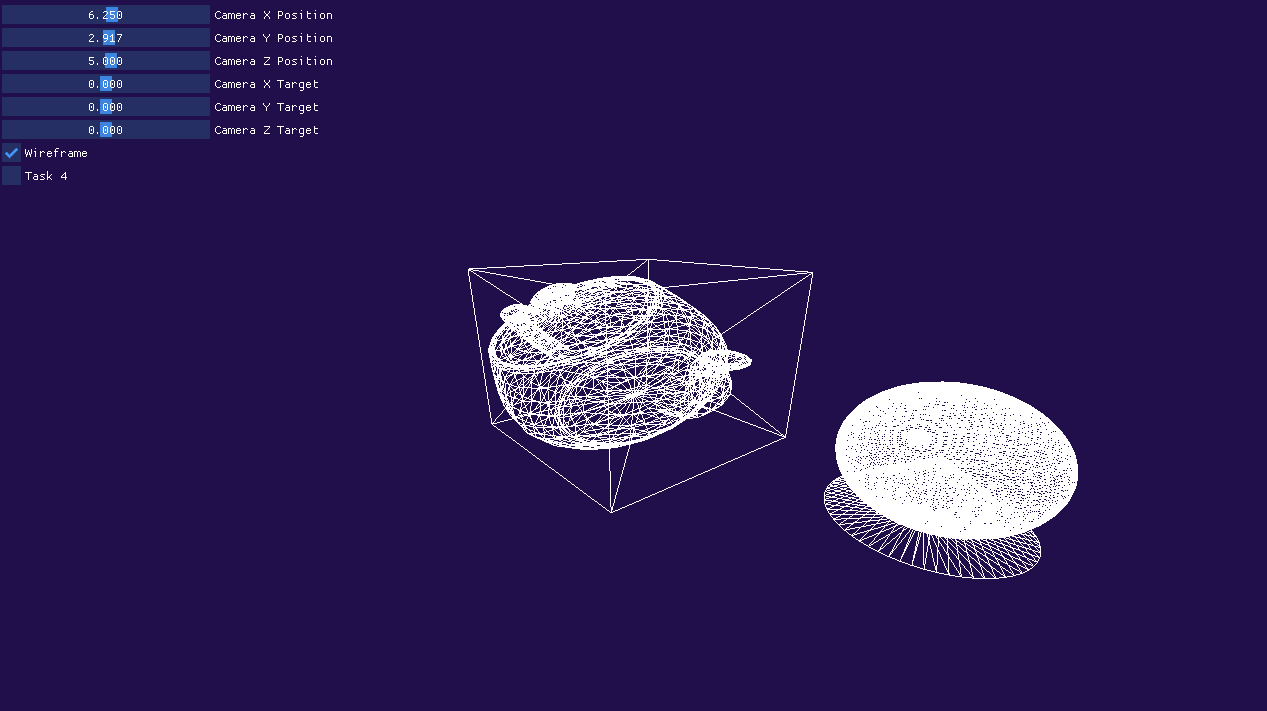
\includegraphics[width=\textwidth]{images/image.1.png}
    \caption{Сцена с другого ракурса}
\end{figure}
\begin{figure}[H]
    \centering
    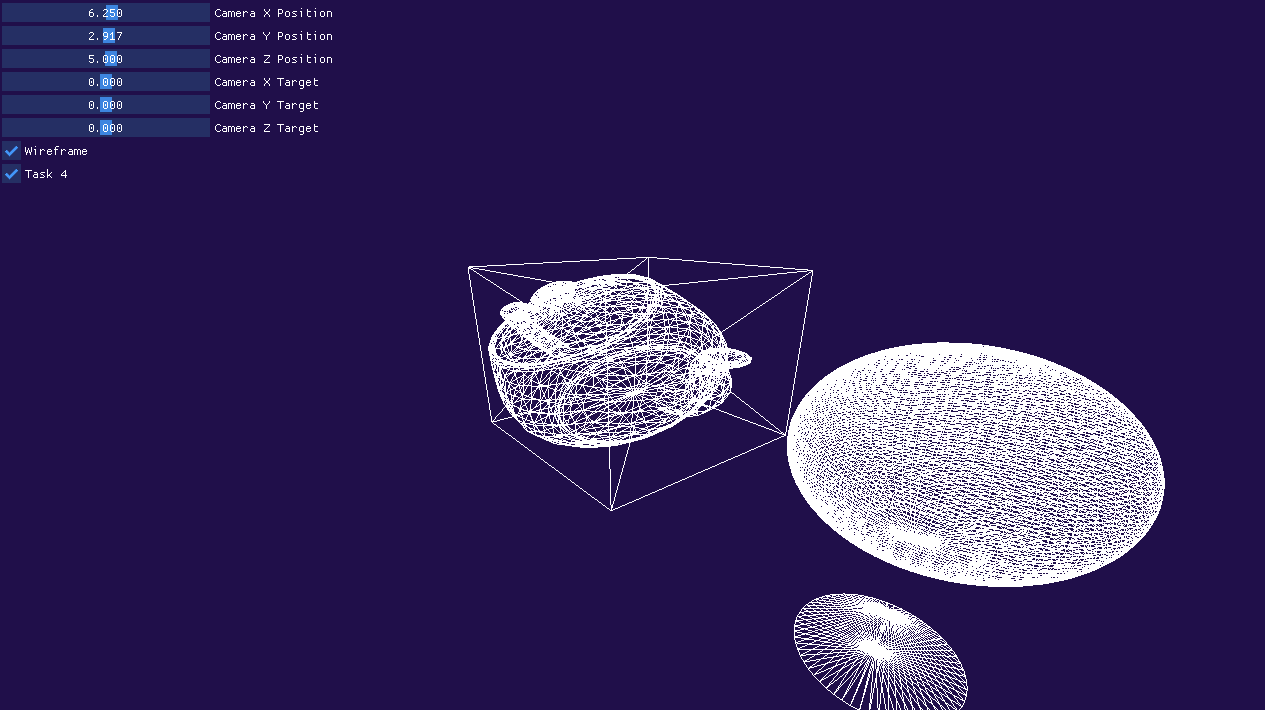
\includegraphics[width=\textwidth]{images/image.2.png}
    \caption{Выполненный пункт 4 из задания}
\end{figure}
\newpage
\subsection*{Исходный код работы}

\subsubsection*{Application.cc}
\lstinputlisting{../../engine/src/c++/application/application.cc}
\newpage

\subsubsection*{Camera.cc}
\lstinputlisting{../../engine/src/c++/camera/camera.cc}
\newpage

\subsubsection*{Material.cc}
\lstinputlisting{../../engine/src/c++/material/material.cc}
\newpage

\subsubsection*{Object.cc}
\lstinputlisting{../../engine/src/c++/object/object.cc}
\newpage

\subsubsection*{RenderObject.cc}
\lstinputlisting{../../engine/src/c++/object/render_object.cc}
\newpage

\subsubsection*{Mesh.cc}
\lstinputlisting{../../engine/src/c++/mesh/mesh.cc}
\newpage

\subsubsection*{OBJMesh.cc}
\lstinputlisting{../../engine/src/c++/mesh/objmesh.cc}
\newpage

\subsubsection*{Cube.cc}
\lstinputlisting{../src/c++/cube.cc}
\newpage

\subsubsection*{Cone.cc}
\lstinputlisting{../src/c++/cone.cc}
\newpage

\subsubsection*{Sphere.cc}
\lstinputlisting{../src/c++/sphere.cc}
\newpage

\subsubsection*{main.cc}
\lstinputlisting{../src/c++/main.cc}
\newpage
\end{document}
